\documentclass[aspectratio=169]{beamer}
\usetheme{Bruno}
\usepackage{amsmath}
\usepackage{amssymb}
\usepackage{siunitx}
\usepackage{float}
\usepackage{tikz}
\def\checkmark{\tikz\fill[scale=0.4](0,.35) -- (.25,0) -- (1,.7) -- (.25,.15) -- cycle;} 
\usepackage{url}
\usepackage[siunitx,american,RPvoltages]{circuitikz}
\ctikzset{capacitors/scale=0.7}
\ctikzset{diodes/scale=0.7}
\usepackage{tabularx}
\newcolumntype{C}{>{\centering\arraybackslash}X}
\renewcommand\tabularxcolumn[1]{m{#1}}% for vertical centering text in X column
\usepackage{tabu}
\usepackage[spanish,es-tabla,activeacute]{babel}
\usepackage{babelbib}
\usepackage{booktabs}
\usepackage{pgfplots}
\usepackage{hyperref}
\hypersetup{colorlinks = true,
            linkcolor = black,
            urlcolor  = blue,
            citecolor = blue,
            anchorcolor = blue}
\usepgfplotslibrary{units, fillbetween} 
\pgfplotsset{compat=1.16}
\usepackage{bm}
\usetikzlibrary{arrows, arrows.meta, shapes, 3d, perspective, positioning}
\renewcommand{\sin}{\sen} %change from sin to sen
\usepackage{bohr}
\setbohr{distribution-method = quantum,insert-missing = true}
\usepackage{elements}
\usepackage{verbatim}
\usetikzlibrary{mindmap,trees,backgrounds}
 
\definecolor{color_mate}{RGB}{255,255,128}
\definecolor{color_plas}{RGB}{255,128,255}
\definecolor{color_text}{RGB}{128,255,255}
\definecolor{color_petr}{RGB}{255,192,192}
\definecolor{color_made}{RGB}{192,255,192}
\definecolor{color_meta}{RGB}{192,192,255}
\usepackage[edges]{forest}
\usepackage{etoolbox}
\usepackage{schemata}
\newcommand\diagram[2]{\schema{\schemabox{#1}}{\schemabox{#2}}}
\title{Instrumentación II: \\ \emph{Estructuras de}\\ \emph{datos}}
\author{Juan J. Rojas}
\institute{Instituto Tecnológico de Costa Rica}
\date{\today}
\background{fig/comunes/background.jpg}
\begin{document}
% \sisetup{unit-math-rm=\mathrm,math-rm=\mathrm} % change sinitx font
\sisetup{output-decimal-marker = {,}}
\maketitle

\newcommand{\blackandwhite}{white} %change this at the end

\begin{frame}{}
\begin{center}
    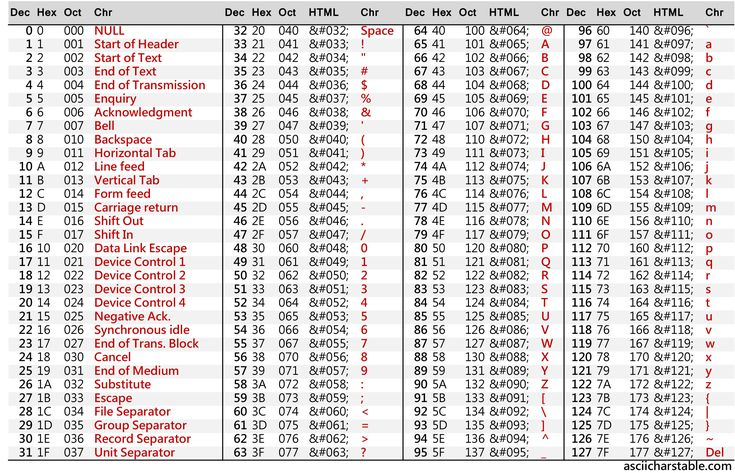
\includegraphics[width=0.93\linewidth]{fig/ASCII.jpg}
\end{center}

\end{frame}

\begin{frame}{Cadenas de caracteres}
Secuencia de caracteres ASCII. Se representan en color rosa en LabVIEW
Funciones: 
\begin{itemize}
    \item Mensajes de texto
    \item Controlar instrumentos por medio de comandos
    \item Recibir información de instrumentos
    \item Almacenar datos numéricos en archivos
\end{itemize}
\begin{tikzpicture}[overlay,remember picture]
        \node[left=0.5cm] at (current page.25){
            
\includegraphics[width=2cm]{fig/string_data_type.png}
        };
\end{tikzpicture}
\end{frame}


\begin{frame}{Referencias}

\bibliographystyle{ieeetr}
\footnotesize
\bibliography{comunes/referencias}

\end{frame}

\end{document}